\documentclass[11pt,a4paper]{article}

%--------------------
% Packages
% -------------------
\usepackage[utf8x]{inputenc}
\usepackage{CormorantGaramond}
\usepackage{orcidlink}
\usepackage[english]{babel}
\usepackage[natbib=true,backend=biber,sorting=nyt,style=apa]{biblatex}
\usepackage[a4paper, lmargin=0.1666\paperwidth, rmargin=0.1666\paperwidth, tmargin=0.1111\paperheight, bmargin=0.1111\paperheight]{geometry}
\usepackage{fancyhdr}
\renewcommand{\baselinestretch}{1.35}
\usepackage{svg}
\usepackage{amsmath}


% Doument setup
\hypersetup{
    colorlinks=true,
    urlcolor=blue,
    linkcolor=black
}
\setlength{\parindent}{4em}
\setlength{\parskip}{1em}
\frenchspacing

\fancyhf{}
\fancyhead[L]{\textbf{UZH – Department of Political Science}}
\fancyhead[R]{Bachelor's thesis}
\fancyfoot[L]{Timothy Justin Oesch}
\fancyfoot[R]{\thepage}
\renewcommand\headrulewidth{0pt}
\pagestyle{fancy}

\usepackage{etoolbox}
\AtBeginEnvironment{quote}{\par\singlespacing\small}

%Footnote definition
\makeatletter 
\renewcommand{\@makefntext}[1]{
    \setlength{\parindent}{0pt}
    \begin{list}{}{
    \setlength{\labelwidth}{1.5em}
    \setlength{\leftmargin}{\labelwidth}
    \setlength{\labelsep}{3pt}
    \setlength{\itemsep}{5pt}
    \setlength{\parsep}{0pt}
    \setlength{\topsep}{0pt}
    \footnotesize}
    \item[\@makefnmark\hfil]#1
    \end{list}
}
\makeatother

\begin{document}
\begin{titlepage}
\title{
    \raggedright
    \small
    \textsc{Bachelor's Thesis} \\
    \vspace{0.5cm}
    \fontsize{25pt}{25pt}
    \textbf{Playing Moneyball}\\
    \vspace{0.2cm}
    \Large\textit{Analyzing the influence of election campaign budgets on the media agenda and electoral outcomes} \\
    
    \vspace{1cm}

    \textbf{Timothy Justin Oesch \orcidlink{0000-0002-4302-5086}}\\
    \vspace{0.25cm}
    \normalsize
    \textbf{Student ID:} 18-719-187\\
    \textbf{Address:} Agnesstrasse 42, CH-8004 Zürich\\
    \textbf{E-mail:} \href{mailto:timothyjustin.oesch@uzh.ch}{\underline{timothyjustin.oesch@uzh.ch}}\\
    
    \vspace{0.5cm} 
    Written in the seminar\\
    \textit{«Agenda-settig: How do issues get important?»}\\
    Module ID: 24FS/23HS 615-BAa
    
    \vspace{0.5cm}
    Written under the supervision of\\
    \textbf{Dr. Jonathan Klüser PhD}

    
    
    \vspace{0.25cm}
    \scriptsize{
        Word count: XXXXXXX \\
        Submission date: June 1, 2024
    } \\
    
    \date{}
    \begin{figure}[b]
        \centering
        
\includegraphics[width=200px]{LaTeX/partials/01.1_uzh_logo.png}
    \end{figure}
}
\clearpage\maketitle
\thispagestyle{empty}
\end{titlepage}

\newpage
\pagestyle{fancy}
\pagenumbering{gobble}
\tableofcontents

\newpage

\listoffigures
\listoftables

\newpage

\pagenumbering{roman}

\begin{abstract}
    Amet aliquam id diam maecenas ultricies mi eget. Fringilla phasellus faucibus scelerisque eleifend donec pretium vulputate sapien nec. Lectus urna duis convallis convallis. Sem et tortor consequat id porta nibh venenatis cras sed. Ultricies tristique nulla aliquet enim tortor at auctor. Feugiat pretium nibh ipsum consequat nisl vel pretium lectus. Ac feugiat sed lectus vestibulum mattis ullamcorper. Felis donec et odio pellentesque diam volutpat commodo. Aliquam sem et tortor consequat id porta nibh venenatis cras. Sed enim ut sem viverra aliquet. Vel quam elementum pulvinar etiam non quam.
\end{abstract}

\section*{A well-known puzzle: Elections, campaign funds, and the media.}
\addcontentsline{toc}{section}{\protect\numberline{}A well-known puzzle: Elections, campaign funds, and the media.}

One of the few times the general public gets into contact with political scientists is during election season and on election days: Pundits, experts and analysists all try to explain why a campaigning party or individual is behaving in a certain way and, when the deed is done, they will contextualize the results, predict the consequences of the electoral outcomes and, in light of surprising results, try to decipher which factors were causal for the loss of a sure-set winner or the win of an underdog. This last question, linking supply- and demand-side components, institutional factors and the political landscape to the vote tally, is one of political science’s most interesting and most pressing questions: \textit{Which characteristics contribute to a party’s electoral success? Which contribute to its demise?} A plethora of studies and papers have tried to find answers to these conundrums and yet, electoral surprises are a dime a dozen: Be it the defeat of Hillary Clinton in the 2016 presidential election, Jeremy Corbin’s Labour party exceeding everyone’s expectations in Theresa May’s failed snap election in 2017, or the incredible victory of the \textit{CHP} in Turkey in the country’s most recent local elections. At the time of writing this introduction, exactly 7 days have passed since a gargantuan shift in Turkey’s political landscape took place. In a major upset, the opposition party around Istanbul’s mayor Ekrem İmamoğlu has enjoyed a landslide victory and was able to dethrone Erdoğan’s \textit{AKP} as the outright winner of any national election since the \textit{AKP}’s establishment in 2001: The \textit{CHP }was able to flip 9 constituencies from Erdoğan’s party, leading the BBC to title \textit{«Opposition stuns Erdogan with historic victory»} (Kirby \& Kasapoglu, 2024), quoting president Erdoğan himself as saying that the outcome marked \textit{«a turning point»}. The Foreign Policy Magazine announced that \textit{«Post-Erdogan Turkey Is Finally Here»} (Cook \& Ciddi, 2024), while the Swiss \textit{Tages-Anzeiger} proclaimed that \textit{«Sunday marked the beginning of the end of Erdogan»} (Geiger, 2024). All these cases clearly show that there is much to learn about the inner workings of election outcomes.

In typical Swiss fashion, such crass election swings seem far from realistic in Switzerland; while the outcomes of direct-democratic referenda are at times more unexpected (as a recent example, one can think of the acceptance of a 13\textsuperscript{th} yearly retirement payment by Swiss voters), a system where \textit{«Konkordanz»}\footnote{In simple terms the idea that a large supermajority of parties ought to be represented in governmental decision-making.} is king will inherently lead to more stable election results. The power and potential consequences of elections are therefore easily forgotten.

Party elites are nonetheless eager to investigate how results came to be: When listening to elites and party activists alike, especially among the political left, it seems to be a popular grievance that, since their opponents’ investments into rallying efforts felt substantially larger than their own, their adversaries were able to reach more voters and reach them better. Such explications make intuitive sense: Spend more, get a larger audience. Past research has acknowledged the prevalence of popular beliefs linking campaign funds to electoral outcomes (Milyo, 2015; Sorauf, 1992). As a campaigner and aspiring political scientist myself, I have made the baffling experience that the widespread and undisputed conviction among the general public that financial resources are a central, if not \textit{the} central, factor in determining political success, the state of the sciences is inconclusive. Questions surrounding the effects of campaign funds seem to be another example of where popular belief and scientific evidence diverge.

Another prevalent argument surrounds what I would like to call the \textit{«larger political climate»}: It is evidently important that, for a party to succeed, voters will need to know what a party stands for on the one hand, and on the other, they will need to perceive the issues a party highlights to be relevant. Loosing parties will often argue that they were unable to talk about what was \textit{«on people’s minds»} and they were therefore unable to rally support and mobilize beyond their party’s base. This suggestion touches upon two relevant subjects: \textit{Issue salience} and the \textit{public agenda}. Past literature has held ample debate around how topical importance\footnote{The terms \textit{«importance»}, \textit{«centrality»}, \textit{«ego-involvement»}, and \textit{«salience»} have all been used to describe a concept that is, to the extent of this paper, essentially identical and they will be used interchangeably. For a more nuanced definition, see Krosnick (1988).} shapes a voter’s preferences and there is evidence in favor of the hypothesis that more important issues will have stronger impacts on a voter’s choices (Krosnick, 1988, 1990). Embedding this idea into the research of the analysis hereinafter allows us to ask the question at heart of the field of agenda setting: How do topics become important? More specifically: \textit{Why do people perceive an issue to be the most important one?}

The following pages shall suggest a path forward: Through analysis of the applicable literature, I will propose a mechanism in the field of electoral research that unifies considerations surrounding campaign funds and their effects on the \textit{«political climate»}. This mechanism allows me to stipulate three hypotheses revolving around the nexus of campaign activity and party budgets, its ramifications on firstly the quantitative representation of parties in the media and secondly the substantive topics represented in the media agenda. Put simply: I set out to test whether campaign budgets influence how active a party can be during the election period, which could in turn change how often they appear and how successfully they can situate their issues in the media. I will go on to argue what the consequences of these hypotheses, if true, would be. A novel dataset and the use of an automated coding process of media articles and party programs allows me to test these hypotheses against the backdrop of a recent Swiss election, concluding in summarizing the broader scientific implications of this thesis and highlighting its shortcomings and future research potential.


\newpage
\pagenumbering{arabic}
\section{A trident of knowledge: Relevant scientific literature }
Before digging into the pertinent literature, let me mark off which scientific foundation this thesis is resting on. My approach shall resemble a trident: The first point considers how agenda setting processes shape the way vote choices come into existence. I will thereunto zoom in on the relevance of issue-salience and how it shapes a voter’s perception of electoral options. Moving closer to the key subject of this paper, I will scrutinize the conjunction of topic relevance and the media. The second point will discuss, if and how political actors are trying to influence the media agenda. The third and last point shall scrutinize the current state of campaign budget research, highlighting nuances in a diffuse debate. 

\subsection{The first prong: Does issue-salience matter?}
\subsubsection{Chasing causality: A brief outline.}
As it would amount to hubris to claim this thesis could summarize a field of research as tremendously large as the one concerned with explaining vote choices, I will rely on the summarizing work by Kulachai et al. (2023). The authors group the mechanisms they identified into three sections: Individual-level, socio-cultural and political explanations. 

While the individual-level reasonings include socioeconomic/-demographic elements (age, gender, education and income) and intrapersonal factors (political ideology, personality traits and emotional intelligence), I want to highlight the fact that Kulachai et al. group two political issues into these explanations: \textit{«Healthcare Experiences»} and \textit{«Climate Change Concerns»}. I want to argue the notability of this by emphasizing that in both cases, the authors attach voting behavior to the mechanisms through the issue’s salience: Whereas the COVID-19 pandemic put topics surrounding the healthcare system in the limelight and the \textit{«urgency of addressing climate change has become increasingly salient among voters»}, these two subjects have become overarching determinants of voting behavior. The second and third group of rationalizations in the article include a potpourri of cultural and political factors, of which I will address a few in the following subchapters.

\subsubsection{Honing in on issue salience.}
As the likely most significant study – and arguably the most comprehensive case against the impact of issue positions and salience on vote choices – Kulachai et al. mention \textit{«The American voter» }(A. Campbell et al., 1960). In this influential seminal study, the authors popularized the Michiganian view of vote choices where partisan identification is far and beyond the strongest predictor of electoral behavior. Yet, I want to call the validity of this theory for the analysis at hand into question: Firstly, the case is heavily centered around the American political system and questionably applicable in other contexts, and secondly there has been significant scientific opposition, exemplified by Key’s infamous quote that \textit{«voters are not fools»} (Key, 1966).

In his 1988 paper, Krosnick reassesses the arguments in the domain of issue salience and their impact on vote choices and delivers a mechanism in which this effect might manifest itself. He finds evidence that the centrality voters assign to issues does potently determine how they evaluate candidates and their voting behavior. Krosnick proposes that this is a result of the fact that more important issues are more readily available in voters’ memories, and they seem to be able to differentiate candidates more easily on these topics. In 1990, he states further that voters’ salient attitudes are highly resistant to change (Krosnick, 1990).

Fournier et al. (2003) expand on Krosnick’s work by linking issue importance to governmental performance evaluations (another popular determinant of voting behavior) and – for this paper more importantly – through a theoretical discussion of problem salience in the domain of agenda-setting. The authors contest that the array of topics that voters will use to evaluate electoral options is not all encompassing. They posit that, due to \textit{«human cognitive limitations»}, voters will inevitably focus on the evidence that comes to their minds easily and quickly. The fundament of these considerations can be found in the book section by Miller and Krosnick (1996): The authors paint voters’ attitudes as a network of mental nodes with a relative strength which is determined by how frequently that node has been activated: \textit{«The more one has thought about an attitude in the past, the stronger its node will be»}. Subsequently, the stronger a node, the more readily available its information will be and, in accordance with Fournier et al., the more influential it will be when casting a vote. Delineating from traditional persuasion, where factors influence the substantive position voters hold, agenda-setting and priming are the processes where actors influence said node-strength.

\subsubsection{The forth estate and its powers: Linking issue-salience to the media.}
Taking the next step in this endeavor, it is now time to turn to who these actors are. Using an at the time innovatory experimental setting, Iyengar and Kinder (1987) deliver indubitable evidence to how the news media influences political priorities. By unrecognizably altering news broadcasts, adding stories concerned with either national security or unemployment into their midst and presenting two groups of volunteers with one of the versions, they were able to show that subjects exposed to more national security content were more likely to rate national security as a higher political priority and vice versa. 

They thereby lay credence to Cohen’s claim that the media \textit{«may not be successful much of the time in telling people what to think, but it is stunningly successful in telling its readers what to think about»} (Cohen, 1964). These experiments and the four studies in Miller and Krosnick (1996) strongly support the framework proposed by McCombs and Shaw: In their paper, they make a succinct case that the electorate does turn to mass media for political information. They analyze the agenda setting function of mass media in-depth, finding a substantial correlation between the foci of the mass media and the public at large. While the authors were hesitant about their findings, the context provided in the years since the study’s publication lead me to contend that, indeed, \textit{«voters do learn»} (McCombs \& Shaw, 1972).


\subsubsection{Summary and implications}
Before examining the ways in which political actors will try to influence the media, I shall briefly recap the submitted knowledge so far and its implications for this paper: The literature shows that issue salience is a significant determinant of voting behavior and delivers a cognitive causal pathway. Papers by Krosnick et al. and Fournier et al. provide mechanisms in which salience is determined by agenda-setting processes and priming effects. Lastly, the publications by Iyengar and Kinder and Miller and Krosnick revealed – in laboratory as well as natural survey settings – that media actors significantly influence which topics become central in voters’ minds and which don’t. The significance of these findings cannot be overstated: While the general reader might already hold the belief that the news media shapes our political landscape profoundly – or as Schudson (1988) put it in his review of Iyengar and Kinder: \textit{«Why should it take fourteen laboratory experiments in Ann Arbor and New Haven, involving more than l ,000 participants from all walks of life, conducted over a four-year period from 1980 through 1983, to demonstrate the obvious?»} – providing omnifarious and indubitable scientific evidence for this commonsense belief is one of the cornerstones of my analysis. 


\subsection{The second prong: Do politicians matter?}
The second and third part in this review of the scientific literature are more narrowly circumscribed but I’d argue just as important as the first one. I will now turn to the question: \textit{What does the state of the sciences say about political actors’ influence on the media agenda?} 


\subsubsection{Are we human or are we dancer?}
I want to argue this conundrum through two opposing camps in line with the distinction proposed by Beckett (1994): In her paper, Beckett analyzes how the «Street crime»-issue became part of the public agenda, identifying the \textit{objectivist model} and the \textit{constructionist model }as possible explanations. Proponents of the objectivist account argue that a social problem, i.e. phenomena that influence social well-being (Manis, 1974), will become a part of the political discourse largely independently from subjective interference. In this narrative, impartial cognizance of the situation around an societal state is a \textit{«necessary and largely sufficient condition for the identification of a social problem.»} In addition, objectivists posit that political action is a result of reactionary problem solving as opposed to proactive shaping of public opinion. Constructionists set forth the idea that, in order for social conditions to become part of the public interest, reality must be interpreted through the use of frames (Hall et al., 1978). They believe that an abundance of actors compete for which of these frames will become part of the political hegemony (Edelman, 1988; Gamson et al., 1992) by drawing attention to specific aspects of the problem they are advocating for. 

Beckett goes on to differentiate between \textit{culturalist} and \textit{elite constructionism}. While this distinction might seem pedantic, it is, I’d argue, at the heart of the mechanism I am proposing: While culturalist-constructionists agree with the framing-principle, thereby disagreeing with objectivists on the root causes of why an issue becomes part of the agenda, they still see political action as the result of public opinion. Elite-constructionists on the other hand propose that political elites – facilitated by the news media’s need for credible or \textit{«institutional»} sources – will be the ones who get the ball rolling, or as Bennett (1980) puts it: \textit{«[…] the general public is most often called on by interest groups and elites to participate in the debate about issues that have already been defined.»} This means that in an elite-constructionist world, political activity is not the consequence, but the cause of public opinion. Beckett, notably, also calls this distinction a «pluralist v. agenda-setting» discussion.

Beckett goes on to test 4 hypotheses, providing significant evidence in favor of the agenda-setting, constructionist account. In summary, the assumption that her findings are independent of the specific social topic implies that it is political and media elites who will shape the public agenda. Conversely, Wasow (2020) acknowledges that the scientific consensus gathers around a constructivist worldview, but proclaims the debate over elite- or culturalist constructivism unresolved even more than 2 decades after Beckett’s paper.

\subsubsection{Political activity and the media.}
For the purpose of this paper, I will abstain from debating this point, incorporating elite-constructionism as a premise of my framework. In the concluding remarks, I will discuss the consequences if this conjecture is erronious and suggest a solution for future research. I believe it to be more fruitful to ask not \textit{if} elites influence the media but \textit{how} they would do such a thing. Presuming that campaigning parties deem it necessary to get voters to think about issues at the core of their program, also referred to as \textit{owning issues}\footnote{For a description on issue ownership, see Petrocik (1996) and Stubager (2018).}, they will invest their campaign resources accordingly. It makes intuitive sense that, in order to get in front of as many eyes and into as many minds as possible, campaigners will among other things use the ampflying effects of traditional media outlets. Drawing on research in the field of media studies, Patro et al. (2018) describe how universities will use widespread tendencies in the human psyche by exaggerating scientific findings for their publications to gain traction in the media, finding that half the press releases of specific universities employ such strategies. For the lack of this kind of scrutiny in the field of political communication, I would instead argue that if even universities – citadels of integrity as they claim to be – (ab)use our inate human affinity for sensational claims, actors running for office are not likely to refrain from doing so. The broader illations of this assumption will become clear once we turn to specifying the mechanism and operationalizing campaign activity in the respective chapters.


\subsection{The third prong: Does money matter?}
Before proceeding to answer the titular query of this part, I want to ask a meta question: \textit{Why does it matter if money matters?} Let’s assume that there was scientific consensus in favor of a causal link between financial ability and electoral success: If that was the case, I argue it would be reasonable to urge lawmakers to pass a regulatory framework governing \textit{who} is allowed to spend \textit{how much} money \textit{within which ruleset}. The subjunctive formulation attests to the fact that, in Jeffrey Milyo’s words, the study of campaign finance is \textit{«more notable for its faults and oversights than for its contributions»} (Milyo, 1999). In my point of view, this is one of the reasons why countries such as Switzerland have yet to adopt comprehensive laws governing campaign finances. This chapter will try to give a brief rundown of publications in favor and against an etiological linkage of gold and gain and make a case for why further research will be justified even if all arrows point to no connection.

\subsubsection{Standing on vertigo-inducing shoulders: Inconclusive evidence about money in politics.}
I would be remiss if I did not mention the extrordinary works of Gary Jacobs and Peverill Squire: Their publications expertly summarize the field’s findings (Jacobson, 1985; Squire, 1995). While both authors focus exclusively on US-elections, I see no reason why the findings they present would not be able to serve as guiding principles. One significant argument is, that if we are able to explain voting behavior through campaign-datached factors, most prominantly the state of the economy, there is no room left for campaigns to make a difference. Past research has made conflicting findings on whether economic performance sufficiently determines electoral outcomes,\footnote{In favor: Born (1986); Carson \& Jacobson (2024); Lewis-Beck \& Rice (1992), against: Alesina \& Rosenthal (1989); J. E. Campbell (1997); Erikson (1990).} notably being unable to port aggregate-level findings to the individual level.

To reconcile these difficulties, studies have resorted to investigating the effects of which information voters \textit{have access to}, \textit{retain} and \textit{utilize} to make a decision. The argument summarized in Converse (1962) proclaims the existence of a \textit{floating voter}: An individual with little information and involvement, susceptible to changing their preferences based on campaign activity. Yet again, the derived hypotheses are hotly debated. Zaller (1989) qualifies the theory, introducing the notion of \textit{«differential information flow»}, finding that different levels of campaign intensity and voters’ prior partisan attachment can lead diverse voter groups to be influenced by campaign activity.

The last point I want to shed light upon is the discussion whether regulating campaign finances – the practical implication of any study of money in politics – is justified in its own right. As multiple authors have pointed out, the restriction of spending can be thought of as a restriction on free-speech rights (Kang, 2012; Ortiz, 1998) and as such must follow the ideas of necessity, proportionality and suitability. Cordis and Milyo (2013) and Milyo (2012) have analyzed if limiting funds has reduced public corruption and increased public trust in government respectively, both finding no significant relation, calling the suitability of such measures into question.\footnote{Notably, it is unclear if the 2012 paper was subject to peer-review as it was published on the Social Science Research Network SSRN. Similarly note-worthy is the provenance of the 2013 study, as it was published under the patronage of George Mason University, an institution that was widely criticized for accepting significant financial support by conservative billionaires like Charles Koch (Larimer, 2018).} Fouirnaies and Fowler (2022) showed that, in general, financial contributions of the insurance industry have little effect on public policy, leading one to challenge the necessity of campaign finance laws. Since proportionality is subject to interpretation and both necessity and suitability of campaign finance regulation seem to be questionable, the case against campaign finance regulation is likely strong. In light of recent events, one could argue: \textit{If the glove don’t fit, you must acquit}.


\subsubsection{Empiricism over morality: Bridging a gap.}
Having completed this brief treatise on the relevance of financial campaign resources, it is now time to approach a superordinate dillemma: Jeffrey Milyo (1999, 2015) argues that \textit{«no collective decision rule can always satisfy a certain reasonable set of “rationality” conditions»}. In his 2015 paper, he goes so far as to say that because \textit{«democratic processes cannot be expected to produce policies that are rational or just»}, it is unreasonable to discuss the question of how money influences politics against the backdrop of morality or justice. Although the validity of this morally nihilist argument might seem dubious, Milyo argues that the question on campaign finance regulation must take place in an empirical setting. Hertig (1982) analyzes the influence of campaign budgets on Swiss direct democratic votes and finds heavy skewedness of campaign resources between political camps. In opposition of Milyo’s belief, he concludes:
\begin{quote}
\textit{[...] but even if we were to overestimate the potential and actual effect of pure voting propaganda on the decision-making of voters, the identified advertising structure is still reason enough to critically question the balance of power that prevails in the formation of opinion prior to votes.\footnote{ Hertig is using voting propaganda as a proxy for campaign budgets, an established best practice for the Swiss case, since concrete financial data has been lacking until today. Translated from German, see the original text (p.56) for literal quote.}}
\end{quote}
In his monograph, Sorauf (1992) reviews the situation of campaign finance regulations in the US of the time, concluding in two chapters where he proposes several ways forward for campaign finance reform. One striking element of these last two chapters are his stands on the influence of \textit{political action committees} (PACs): He claims that, since there is no evidence linking «PAC-money» to outcomes regarding public policy, there is not enough reason to ban or even just limit these forms of political organization. In a tough-but-fair review of his work, Gross (1993) calls this the «Burden of Proof Question», highlighting that Sorauf places this burden on the individuals trying to reform campaign finance law. Gross emphasizes that there are \textit{«different and disproportionately important consequences of placing the burden of proof in the wrong place»}. Gross concedes that \textit{«one typically works on the assumption that the burden of proof is on those trying to establish a relationship»}, but because of the immense complexity of finding empirical evidence for the influence of PAC-money and the fatal consequences of falsely assuming there to be no connection, it is reasonable to put the burden-of-proof on those arguing against campaign finance restriction. In a time where the courts, established in \textit{Citizens United v. Federal Election Commission} (2010) and \textit{SpeechNOW.org v. Federal Election Commission} (2010), have essentially allowed so called «super PACs» to raise and spend a practically unlimited amount of money\footnote{ As long as they do not coordinate with stakeholders such as candidates they are supporting, a fact that has become a practical joke in popular culture.} in the US based on free speech considerations, one can only wonder if Frank Sorauf would still believe in his position as he passed away only 3 years after the decisions were published.

This is the exact context in which this study takes place; the crossroads between empirical observations and questions of morality, ethics, and justice. It is the prescribed goal of the analysis to test whether there is a so far missed link between campaign spending and electoral outcomes through the means of issue-salience and, therefore, regulations for campaign finance are justified, not just when scrutinizing them philosophically, but also empirically.


\section{Framework and empirical implications}

\subsection{The case for a new model.}

\subsubsection{Making Money Moves: Three steps from cash to conversation.}
The model set out to be tested can be stylized as depicted in Figure 1. \textit{Campaign funds} are connected to a \textit{party’s resources} intuitively: The more money a party can invest into an election campaign, the more people that party can engage professionally, the larger their ad-buy, the more resources they have at their disposal to do communication research, content creation, activist mobilization and more. This leads the party to be a more potent influence on the agenda-setting process through \textit{campaign activity}. 

\begin{figure}[htbp]
    \centering
    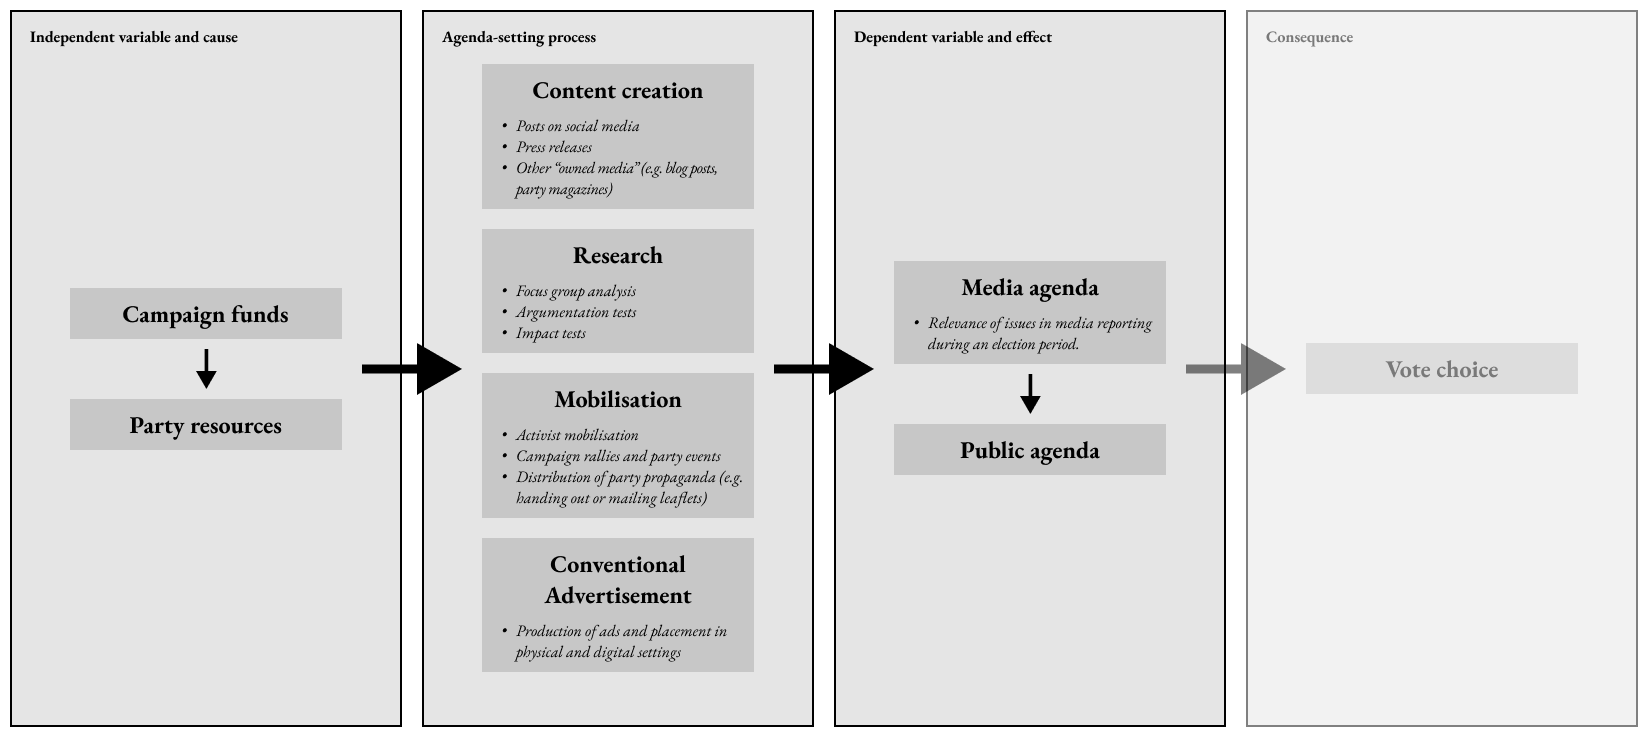
\includegraphics[width=1\linewidth]{LaTeX/figures/Process.png}
    \caption{Proposed mechanism linking campaign funds to the public agenda through campaign activity.}
    \label{fig:enter-label}
\end{figure}
The next step, connecting the agenda-setting process to the \textit{media and public agenda}, is grounded in two premises: Firstly, political elites are assumed to want to be \textit{«as relevant as possible»}, meaning they want to make their parties and their issues visible. In my view, subscribing to this idea in line with the principle of rational utility-maximizing actors is in this case unproblematic. Secondly – as noted and justified above – the mechanism relies on the concept that the public agenda is shaped by \textit{elite-constructivism}, meaning that voters turn to the media to make sense of the world around them (hence constructivism) and the media takes cues from political elites to decide which issues to highlight in their reporting (hence elitism). The crux in this presumption lies not in the constructivist but the elitist aspect, a dispute which this paper will not be able to weigh in on. But even if one believes in a more pluralist worldview, there is room for an alternative mechanism: Such reflections can be incorporated in the position that the more money a party has, the more easily they can \textit{conform to} the public discussion rather than set the public agenda.\footnote{ In the conclusion to this paper, I am proposing a way in which this analysis could be amended in order to lay credence to an elitist pathway.}

The last portrayed step from the public agenda to the electoral result is an implicit one: As shown above, the scientific debate around the influence of issue salience on vote choice is far from settled. Even though this paper does not aim to add to this controversy directly, I find it relevant to keep an eye on the bigger picture and suggest that future research traces the machinery I proposed all the way to electoral outcomes, as this is where the most practical implications in regards to policymaking lie.


\subsubsection{Putting flesh on the bone: Hypotheses.}
I am now ready to propose three hypotheses that can be derived from my framework.
\textit{The agency hypothesis (H1):} My framework suggests that the higher a campaign’s resources, the larger their campaign output to set the public agenda. My first hypothesis should therefore read: \textit{The higher a party’s election campaign budget, the more active they are during an election campaign.}

\textit{The frequency hypothesis (H2):} The second implication of my model is, that campaigning parties want to be as salient as possible in the time leading up to an election in order to be atop voters’ minds. In order to achieve this, they will try to appear in the media as frequently as possible. The second hypothesis I therefore present goes: \textit{The higher a party’s election campaign budget, the more frequently they will appear in media reporting.}

\textit{The issue salience hypothesis (H3):} The third and final derivative I take away from my machinery surrounds the centrality of issues in the media agenda. If parties are competing for the issues they put at the forefront of their program to take up space in the media and campaign activity has an effect on the news’ content, then there should be a correlation between campaign budgets and media issue salience. This leads me to claim: \textit{The higher a party’s election campaign budget, the more likely it is that the issues that are relevant for them are relevant in the media agenda as well.}

\subsection{Empirical implications: What should we observe?}
Before moving on to test these claims, I will here delimit which observations would underpin them. Support for H1 would be if the quantity of campaign activity rose in tandem with campaign budgets. In other words: It would aid H1 if parties are campaigning more vigorously when they have higher budgets. For H2 to be validated, we would need to see an analog rise in party occurrence in media reporting correlating with campaign budgets. While the expected evidence for H1 and H2 is rather intuitive, H3 is a harder nut to crack: For me to establish a relationship between campaign budgets and issue salience in the media, I propose to analyze the effect of the interaction between issue salience for a party and that party’s campaign budget on the salience of the issue in the media. Put simply: The best evidence for H3 is, if the topics important to a party with a high campaign budget are more salient in the media than the topics important to a party with a low campaign budget.


\section{Empirical analysis}

\subsection{Case selection}
As previously hinted to, my analysis surrounds the Swiss national elections of 2023 for the larger chamber of parliament. This case is suitable in several regards: Firstly, there is novel data available for the campaign funding. For the first time in Swiss history, all parties and interest groups were obligated to transparently provide how much money they fundraised during the election and which candidates benefited from it. Secondly, Switzerland is the only member state of the Council of Europe to have practically no restrictions on political financing (Jaberg, 2019): Such restrictions could skew our analysis. Lastly, the key-metrics of average swing and turnout were nominal for the 2023 election as shown in Table 1 and Table 2: The average party-swing was at around 1\%, while turnout was at 46.6\%.


\begin{table}
\centering
\caption{Swing calculations for the Swiss federal elections from 1999–2023 with a 24-year-average swing of 1.45\% and a 24-year-median swing of 1.57\%.}
\vspace{0.5cm}
\label{tab:my_table}
\begin{tabular*}{\linewidth}{@{\extracolsep{\fill}} | l | l | l | l | l | l | l | l | }
\hline
\textit{Party}\textbf{ / Year} & \textbf{2023} & \textbf{2019} & \textbf{2015} & \textbf{2011} & \textbf{2007} & \textbf{2003} & \textbf{1999} \\
\hline
\textit{SVP} & +2.3\% & –3.8\% & +2.8\% & –2.4\% & +2.2\% & +4.2\% & +7.7\% \\
\hline
\textit{SP} & +1.5\% & –2.0\% & +0.1\% & –0.9\% & -3.7\% & +0.8\% & +0.7\% \\
\hline
\textit{FDP} & –0.8\% & –1.3\% & +1.3\% & –2.5\% & -1.5\% & -2.6\% & -0.4\% \\
\hline
\textit{Mitte} & +0.2\% &   &   &   &   &   &   \\
\hline
\textit{Grüne} & –3.4\% & +6.1\% & –1.3\% & –1.2\% & +2.2\% & +2.3\% & -0.2\% \\
\hline
\textit{glp} & –0.2\% & +3.2\% & –0.8\% & +4.0\% & +1.4\% &   &   \\
\hline
\textit{EVP} & –0.1\% & +0.2\% & –0.1\% & –0.4\% & +0.1\% & +0.5\% & +/-0\% \\
\hline
\textit{EDU} & +0.2\% & –0. 2\% & –0.1\% & +/-0\% & +/-0\% & +/-0\% &   \\
\hline
\textit{CVP} &   & –0.2\% & –0.7\% & -2.2\% & +0.1\% & -1.4\% & -1\% \\
\hline
\textit{BDP} &   & –1.6\% & –1.3\% & +5.4\% &   &   &   \\
\hline
\textit{LPS} &   &   &   &   & -0.4\% & -0.1\% & -0.4\% \\
\hline
\textit{SD} &   &   &   &   &   & -0.8\% & -1.3\% \\
\hline
\textit{other} & +0.3\% & –0.3\% & +0.1\% & +0.2\% & -0.4\% & -3\% & -2\% \\
\hline
\textbf{Average Swing} & \textbf{1.00\%} & \textbf{1.89\%} & \textbf{0.86\%} & \textbf{1.92\%} & \textbf{1.2\%} & \textbf{1.57\%} & \textbf{1.68\%} \\
\hline

\end{tabular*}

\end{table}


\begin{table}
\centering
\caption{Turnout statistics for the Swiss federal general elections from 1999–2023 with a 24-year-average turnout of 46.56\% and a 24-year-median turnout of 46.60\%.}
\vspace{0.5cm}
\label{tab:my_table}
\begin{tabular*}{\linewidth}{@{\extracolsep{\fill}} | l | l | }
\hline
\textbf{Year} & \textbf{Turnout} \\
\hline
\textit{2023} & 46.6\% \\
\hline
\textit{2019} & 45.1\% \\
\hline
\textit{2015} & 48.4\% \\
\hline
\textit{2011} & 48.6\% \\
\hline
\textit{2007} & 48.8\% \\
\hline
\textit{2003} & 45.2\% \\
\hline
\textit{1999} & 43.2\% \\
\hline

\end{tabular*}

\end{table}

For party selection, we will use all parties that were independently able to build factions in the national council after the election, which leaves us with 6 parties.\footnote{SVP, SP, FDP, die Mitte, GPS (the green party of Switzerland) and glp.}

Which media outlets to be considered seems a bit more complex. The Swiss media landscape is very diverse: There is significant variance in political leaning as well as in regionality. Past research has used the \textit{Neue Zürcher Zeitung} for analysis of agendas, yet focusing on a single newspaper seems unnecessarily narrow. The \textit{Tages-Anzeiger,} the highest circulating fee-based newspaper in the German-speaking part of Switzerland (Presence Switzerland, 2018), shall be added to this list as well as articles published in the online portal of \textit{Schweizer Radio und Fernsehen SRF} and articles of the German edition \textit{20 Minuten}, a free daily newspaper.

\subsection{Methods, operationalization, and dataset preparation.\footnote{ For data and code, see Appendix B.}}
The basis of my analysis shall be the dataset on campaign finances (Swiss Federal Audit Office, 2023) which depicts the amount of money parties either received through donations or invested from their own war chests.\footnote{For discussions on the limitations of this measure, see caveat no. 3 in chapter 5.2.} The party earnings will be used in two ways: For H3, I aggregated the earnings of the federal and cantonal levels as well as earnings from special interest groups and individual candidates together based on which party the candidates are from.\footnote{Because the dataset provided by the Swiss Federal Audit Office use the individual «candidate» as level of analysis and the same earnings can therefore appear in the dataset multiple times, I distributed the earnings equally on all candidates that were declared as «supported by» those earnings. I want to argue this to be the most reasonable estimation, as any other distributetion would have to be justified. A concrete example: The «Thurgauer Gewerbeverband» declared earnings of 82’860 CHF with which they claim to have supported 15 candidates. Each candidate therefore was supported with 5’524 CHF. Four of these candidates were by the SVP, leading me to estimate that the «Thurgauer Gewerbeverband» supported the SVP with 22’096 CHF.}$^{, }$\footnote{This process allowed me to assign a large majority of all earnings-data to parties. This includes parties that are irrelevant for this analysis such as the «EDU». From the 2616 rows in the dataset, only 7 rows were unassignable because they were not listed as either supporting a declarable array of candidates (\textit{«Gruppe von Kandidierenden: Einzelauflistung nicht möglich»}) or a party that was supported with the entirety of the earnings. As an example for these items: The «Klima Allianz» organized a national manifestation on the 30\textsuperscript{th} of September, earning roughly 315’000 CHF from this event. While it would be hard to argue that this manifestation did not come with a subtle push of a specific ideology, it would be equally hard to class the earnings to concrete parties. Because the «Independent» earnings which these rows fall into do not take up a substantial part of total earnings (2.18\%) as depicted in Figure 2, I contest that they had, at most, an insignificant effect on the overall validity of the data I used.} This is necessary, because a large part of campaigning takes place on the subnational level and through interest groups. This is examplified by the share of earnings by a party on the national level on their total earnings: The six relevant parties had an average national to total earnings ratio of 29.32\%,\footnote{ Minimum: 16.47\%, Maximum: 36.65\%, Standard deviation: 7.46\%.} meaning that, on average, 70\% of the earnings came from other sources than their national party coffers. These measures, though, are exactly what I use for Analyses of H1 and H2. Because aggregation of party activity on the subnational level would exceed the confines of this thesis and activities of special interest groups do not fit into H1 and H2 at all, it is necessary to use the same level of analysis for the party earnings.

Campaign activity, needed to test H1, is operationalized as the number of posts made on Instagram and the number of press releases published by parties within 1 month, 3 months and 6 months of the election. Restriction on these metrics will not be sufficient to make sweeping claims but because this operationalization is reasonably easy to implement – in comparison to others such as the number of people the party employs professionally, the number of newsletters it sends out or because of the non-transparency of other social media like the number of posts on platforms such as X-formerly-Twitter – it will suffice for me to analyze H1 descriptively and present conclusions preliminarily.

For all media related data, I am using the \textit{Linguistic Research Infrastructure Swissdox@LiRI}\footnote{For this publication, use was made of media data made available via Swissdox@LiRI by the Linguistic Research Infrastructure of the University of Zurich (see https://t.uzh.ch/1hI for more information).} to pull all relevant articles in the same timeframes as the campaign activity. For H2, we will qualify our queries with the names of the parties and its alternates (eg. \textit{«schweizerische Volkspartei»}, \textit{«Schweizerische Volksparti»} and \textit{«SVP»}), operationalizing \textit{«party relevance»} as the number of results returned for each party, while articles for H3 will be pulled indiscriminately.\footnote{For the list of queries, see Appendix A.}

Regarding the party position, I am using the election platforms or party programs – whichever was more recent at the time of the election – published by the parties themselves. Since the Manifesto Project Database does not include documents for Swiss parties which are more recent than 2019 (Lehmann et al., 2023), I converted the newest publications into machine readable plaintext by hand, removing all irrelevant information such as titles, figures, tables of contents and other visualizing elements.\footnote{The list of publications used with key metrics and publication specific alterations performed can be found in Appendix C.}$^{, }$\footnote{\textit{Note on «Die Mitte»:} This was the only party where a PDF of positions with reasonable recency was unavailable. The PDF stored in the Manifesto Project Database for the former CVP consists of largely congruent material. This and the fact that the results received conformed with expectations gives credibility of the data I used nonetheless.}$^{, }$\footnote{\textit{Note on the «glp»:} The age of their program (almost 9 years) might seem questionable. The party has published a more recent program \textit{«Es ist Zeit - 26 grünliberale Grundsatzpositionen»} which the Manifesto Project Database used to assess the party’s positions. Since this publication is no longer available on their webpage in comparison to the \textit{«Leitlinien»} I used – which is still prominently featured as the first document on the party’s webpage when looking for its positions – I want to argue the newer paper had little to no effect on the public at the time of the election and is therefore not being used here.}

For the different agenda-issues, we will rely on the 21 major agenda topics provided by the master codebook of the Comparative Agendas Project CAP (Bevan, 2019). I am using an \textit{«AI solution for the automated coding of policy agendas»} called \textit{CAP Babel machine }(poltextLAB, 2023) in order to create a sufficiently large dataset, thereby laying the basis of regression models without the need of double-blind human coding.\footnote{This process delivered a prediction on the most likely category with associated softmax scores, essentially measuring the confidence in its prediction. This analysis uses all predictions: The confidence in predictions for the parties was adequately high, whereas using different cutoffs for confidence regarding media article classification did not yield pertinently different results. See files labelled with the «v2.r» suffix in the code repository.} Sebők \& Kacsuk (2021) have tested this method against human coders and found satisfactory results in terms of precision. The media articles will be coded in their entirety, in turn dividing the number of articles within a subject per CAP-topic by the total number of articles within the selected time-period, resulting in a media-issue-salience-index \textit{MISI}.

\begin{equation}
    MISI\ \widehat{=}\ \frac{n_{Articles\ within\ topic\ and\ timeframe}}{n_{All\ articles\ within\ timeframe}}
\end{equation}

Such an index is created for the month leading up to the election day (\textit{MISI\_1m}) as well as 30 days (\textit{MISI\_3m}) and 180 days prior (\textit{MISI\_6m}) to include as control variables.

The party positions will be coded similarly: The character count of the paragraphs within a CAP topic will be divided by the total number of characters of the publication, resulting in a party-issue-salience-index \textit{PISI}.

\begin{equation}
    PISI\ \widehat{=}\ \frac{n_{Characters\ of\ paragraphs\ within\ topic}}{n_{Characters\ of\ entire\ publication}}
\end{equation}

To test H3, a novel data frame is coded with party-topic dyads with the \textit{MISI} and \textit{PISI} of the topic and the party campaign budget. Additional control variables on the party level are added, including information on the party’s position on the GAL-TAN\footnote{Green-alternative-libertarian vs. traditional-authoritarian-nationalist.} and Economy-Left-Right axes (\textit{«party ideological control»}), pulled from the most recent Chapel Hill expert survey (Bakker et al., 2022), as well as the number of elected representatives before the election (\textit{«party strength control»}). 


\subsection{Model specification (H3)}
To test my third hypothesis, I am running an Ordinary Least Squares OLS regression model using the formula

\begin{equation}
    \begin{split}
        \gamma_{MISI\_1m}\ \sim\ \beta_{PISI}\ +\ \beta_{Earnings}\ +\ \beta_{Party\ ideology}\\
         +\ \beta_{Party Strength}\ +\ \beta_{MISI\_3m}\ +\ \beta_{MISI\_6m}\ +\ (\beta_{PISI}\ \times\ \beta_{Earnings})\ +\ \epsilon  
    \end{split}
\end{equation}


\section{Results}

The following chapter is primarily aimed at presenting and tentatively interpreting the results I received from the analyses I performed. More extensive judgment and discussion of limitations will be made in chapter 5. In a first, descriptive step, I am analyzing the data for validity and reliability as well as providing findings for H1 and H2. The second step consists of running several regression models in order to make claims about H3.

\subsection{Descriptive analysis}
Figure 2 depicts the earnings reported divided by party and source, summed up as described above. There are significant differences in levels of earnings with some parties being able to fundraise a lot more financial resources than others. Somewhat strikingly, though, the FDP was the party with the highest earnings over all, while being the party with the third highest party capital investment. The ratio of fundraised earnings\footnote{Monetary earnings + non-monetary earnings + earnings through merchandise + earnings through events.} against party investment was more than 2:1 for the FDP, the only analysis-relevant party where this is the case. As my aggregation method does not distinguish between party- and interest group contributions, this might influence the effectiveness of the money, as one might argue a buck spent by a party has a larger effect on a party’s ability to influience public opinion than a buck spent by an interest group \textit{for} a party. Future research will have to address this by disentangling the data.

\begin{figure}
    \centering
    \includesvg[width=0.75\linewidth]{output/plots/plot_figure_2.svg}
    \caption{Earnings by party and source. Non-monetary earnings, those through merchandise and events were ommitted for legibilty. Parties labelled * are not part of the analysis, as they were not able to form a faction in the large chamber of parliament after election day}
    \label{fig:enter-label}
\end{figure}




\end{document}